%% gpd.tex,  version 14/05/23

%%%%%%%%%%%%%%%%%%%%%%%%%%%%%%%%%%%%%%%%%%%%%%%%%%%%%%%%%%%%%%%%%%%%%%%%%%%%
\section{Groupoids} \label{sec:gpds}


%%%%%%%%%%%%%%%%%%%%%%%%%%%%%%%%%%%%%%%%%%%%%%%%%%%%%%%
\subsection{Basic definitions} \label{subsect:gpd-defs}
\index{groupoid} \index{object!of a groupoid} \index{arrow!of a groupoid}

A \emph{groupoid} is a category in which every arrow is invertible. 
Thus a groupoid $\bbC = (C_1,C_0)$ consists of the following: 
\begin{itemize}
\item
a set $\Ob(\bbC) = C_0$ of \emph{objects}, 
\item 
a set $\Arr(\bbC) = C_1$ of \emph{arrows}, 
\item
source and target maps $s,t : C_1 \to C_0$, so that we write 
$a:u \to v$ whenever $sa=u$ and $ta=v$, 
and we denote by $\bbC(u,v)$ the set of arrows with source $u$ and target $v$, 
\item 
an \emph{identity arrow} $1_u$ at each object $u$, with $s1_u=t1_u=u$, 
\item 
an associative  partial composition $\diamond: C_1 \times_0 C_1 \to C_1$, 
with $a \diamond b$ defined whenever $ta=sb$, such that 
$s(a \diamond b) = sa$ and $t(a \diamond b) = tb$. 
\item 
for each arrow $(a : u \to v)$ an inverse arrow $(a^{-1} : v \to u)$ 
such that $a \diamond a^{-1} = 1_u$ and $a^{-1} \diamond a = 1_v$. 
\end{itemize}
It will often be convenient to omit the symbol $\diamond$ and use simple 
juxtaposition to indicate composition. 
(In our {\GAP} implementation source and target are called 
\emph{tail} and \emph{head}.) 

An arrow $a$ is a \emph{loop} if $ta = ha$. 
The \emph{vertex group} or \emph{object group} at object $u$ is the group 
$\bbC(u) = \bbC(u,u)$. 

A morphism of groupoids, as for general categories, is called a functor. 
\index{functor} \index{morphism!of groupoids} 
Thus a \emph{functor} $\phi = (\phi_1,\phi_0) : \bbC \to \bbD$
is a pair of maps $\phi_1 : C_1 \to D_1$ and $\phi_0 : C_0 \to D_0$ 
such that $\phi_1 1_u = 1_{\phi_0 u}$ and 
$\phi_1(a \diamond b) = (\phi_1a)\diamond(\phi_1b)$ 
whenever the composite arrow is defined. 
It is often convenient to omit the subscripts $0,1$ since it should be clear 
from the context whether an object or an arrow is being mapped. 
A morphism $\phi$ is \emph{injective} and/or \emph{surjective} 
if both $\phi_0,\phi_1$ are. 

\begin{example} 
\emph{A group is a groupoid with a single object (usually written $*$). 
This gives a functor \Groupoid\; from \catGp\; to \catGpd.} 
\end{example}

\begin{example} \label{ex:triv-gpd} \index{trivial groupoid}
\emph{For $X$ a set, the \emph{trivial groupoid $\bbO(X)$ on $X$} 
has $\Ob(\bbO)=X$ and $\Arr(\bbO)=\{1_u ~|~ u \in \Ob(\bbO)\}$. 
We denote $\bbO(\{1,\ldots,n\})$ by $\bbO_n$.} 
\end{example}

\begin{example} \label{ex:unit-gpd} \index{unit groupoid} 
\emph{The \emph{unit groupoid} $\bbI$ has two objects $0,1$ and four arrows. 
The two non-identity arrows are $\iota : 0 \to 1$ 
and its inverse $\iota^{-1} : 1 \to 0$.} 
\end{example}

The \emph{underlying digraph} of a groupoid 
\index{underlying digraph!of a groupoid}
is obtained by forgetting the composition, 
so the objects become vertices, the arrows become arcs, 
while the source and target maps keep their usual digraph meaning. 
A groupoid is \emph{connected} if its underlying digraph is connected. 

\begin{example} \label{ex:tree-groupoid} \index{tree groupoid} 
\emph{The \emph{tree groupoid} $\bbI_n$ has $n$ objects $\{1,2,\ldots,n\}$ 
and $n^2$ arrows $\{(p,q) ~|~ 0 \leqslant p,q \leqslant n\}$ where 
$s(p,q)=p$, $t(p,q)=q$, $(p,q)\diamond(q,r) = (p,r)$, 
and $(p,q)^{-1} = (q,p)$. 
Note that $\bbI_2 \cong \bbI$. 
We also write $\bbI(X)$ for the tree groupoid on a set of objects $X$. 
The underlying digraph of $\bbI_n$ is complete.} 

\emph{The name tree groupoid comes from the fact that a subset of arrows 
which form a spanning tree in the underlying digraph generate the 
whole groupoid using composition and inversion. 
For example, 
taking the subset $X_n = \{(1,p) ~|~ 2 \leqslant p \leqslant n\}$, 
we have $(q,r) = (1,q)^{-1}\diamond(1,r)$.} 
\end{example}

The \emph{product} $\bbC\times\bbD$ of groupoids $\bbC,\bbD$ 
\index{product!of groupoids}
has objects $C_0 \times D_0$, arrows $C_1 \times D_1$, 
and composition 
$(a_1,b_1)\diamond(a_2,b_2) = (a_1 \diamond a_2, b_1 \diamond b_2)$, 
so that $(a,b)^{-1} = (a^{-1},b^{-1})$. 

\begin{example} \label{ex:gp-tree-gpd}
\emph{If $\bbG$ is a group, considered as a one-object groupoid, 
and $\bbI_n$ is the tree groupoid of the previous example, then $\bbC = \bbG \times \bbI_n$ 
may be thought of as the groupoid with $n$ objects $\{1,2,\ldots,n\}$ 
and $n^2|G|$ arrows $\{(p,g,q) ~|~ g \in G, 1 \leqslant p,q \leqslant n\}$, 
with $t(p,g,q)=p$, $h(p,g,q)=q$, 
composition $(p,g,q)\diamond(q,h,r) = (p,gh,r)$, 
and inverses $(p,g,q)^{-1} = (q,g^{-1},p)$. 
A generating set for $\bbG$ is given by 
$\{(1,g,1) ~|~ g \in X_G\} \cup X_n$ 
where $X_G$ is any generating set for $\bbG$. 
Every finite, connected groupoid is isomorphic to a direct product 
of a group and a tree groupoid in this way, and we call such a 
representation a \emph{standard connected groupoid}.}
\end{example}

A groupoid $\bbA$ is \emph{abelian} \index{abelian groupoid}  
if and only if all its object groups are abelian. 

\medskip
We now describe the construction of a free groupoid on a graph. 
Let $D$ be a digraph with vertices $V = V(D)$, arcs $A^+=A(D)$, 
and source and target maps $s,t : A^+ \to V$. 
Let $A^- = \{a^- ~|~ a^+ \in A^+\}$ be a copy of $A^+$, 
and let $A = A^+ \cup A^-$.  
Extend $s,t$ to $A$ by defining $sa^-=ta^+,~ ta^-=sa^+$. 
Consider $A$ as an alphabet with $A^*$ the monoid of words in $A$ 
under concatenation. 
A word $w=a_1^{\epsilon_1}a_2^{\epsilon_2} \ldots a_k^{\epsilon_k} \in A^*$, 
where $\epsilon_i \in \{+,-\}$, is \emph{composable} 
if $ha_i^{\epsilon_i} = ta_{i+1}^{\epsilon_{i+1}}$ 
for all $1 \leqslant i < k$. 
The \emph{free groupoid} $\bbD$ on $D$ is defined by: 
\begin{itemize} \index{free groupoid}
\item 
the object set is $\Ob(\bbD) = V(D)$,  
\item
$\Arr(\bbD)$ is the set of all composable words in $A^*$, 
\item
$s(a_1^{\epsilon_1}a_2^{\epsilon_2} \ldots a_k^{\epsilon_k}) 
   = sa_1^{\epsilon_1}$, 
and $t(a_1^{\epsilon_1}a_2^{\epsilon_2} \ldots a_k^{\epsilon_k}) 
   = ta_k^{\epsilon_k}$, 
\item
$w_1 \diamond w_2$ is the concatenation of $w_1$ and $w_2$, 
defined if the result is a composable word.
\end{itemize} 
A groupoid $\bbD$ is \emph{free} if it is isomorphic to the free groupoid 
on some digraph $D$. 

\medskip \index{subgroupoid} 
A \emph{subgroupoid} $\bbS=(S_1,S_0)$ of $\bbC=(C_1,C_0)$ 
is a groupoid with $S_0 \subseteq C_0$, $S_1 \subseteq C_1$, 
having the same source, target and composition. 
A subgroupoid $\bbS$ is \emph{full} \index{full subgroupoid} 
if $\bbS(u,v) = \bbC(u,v)$ for all $u,v \in S_0$ 
and \emph{wide} \index{wide subgroupoid} 
if $\Ob(\bbS) = \Ob(\bbC)$. 
The \emph{(connected) components} of $\bbC$ are its maximal 
connected subgroupoids, \index{component!of a groupoid} 
with one component $\bbC_i$ for each of the $k$ connected components 
$\Gamma_i$ of the underlying digraph. 
We write $\bbC = \bbC_1 \cup \cdots \cup \bbC_k$.  
A groupoid whose components all have a single object is a 
\emph{union of groups}, \index{union of groups} 
and is said to be \emph{totally disconnected}. 
\index{totally disconnected groupoid} 
We denote by $\ids(\bbC)$ the wide trivial subgroupoid $\bbO(\Ob(\bbC))$. 

\medskip
Given a wide subgroupoid $\bbS \subseteq \bbC$, 
we may define a relation $\equiv_R$ on $\Arr(\bbC)$ by 
$c \equiv_R c' ~\Leftrightarrow~ c = a \diamond c'$ 
for some $a \in \Arr(\bbS)$. 
This is an equivalence relation since: 
\begin{itemize}
\item
$c = 1_{sc} \diamond c$, since $\bbS$ contains 
all the identity loops in $\bbC$,  
\item
$c \equiv_R c' \Rightarrow c=a \diamond c' \Rightarrow a^{-1}\diamond c=c' 
               \Rightarrow c' \equiv_R c$, so $\equiv_R$ is symmetric, 
\item
$(c_1 \equiv_R c_2,~ c_2 \equiv_R c_3) 
 ~\Rightarrow~ (c_1=a_1 \diamond c_2,~ c_2=a_2 \diamond c_3) 
 ~\Rightarrow~ c_1=a_1 \diamond a_2 \diamond c_3 
 ~\Rightarrow~ c_1 \equiv_R c_3$. 
\end{itemize} 
The equivalence classes $\bbS c$ for this relation are called the 
\emph{right cosets of $\bbS$ in $\bbC$}. 
\index{right coset!of a groupoid} 

\medskip
For $u \in \Ob(\bbC)$ the \emph{star} $\Star(u)$ of $u$ is the set 
\index{star!of a groupoid}
$\{a \in \Arr(\bbC) ~|~ sa=u\}$, the set of all arrows with source $u$. 
Similarly the \emph{costar} $\Costar(u)$ of $u$ is the set 
\index{costar!of a groupoid}
$\{a \in \Arr(\bbC) ~|~ ta=u\}$, the set of all arrows with target $u$.
Note that each right coset of $\bbS$ in $\bbC$ is a subset of a costar. 
We may define a second equivalence relation $\equiv_L$ on $\Arr(\bbC)$ by 
$c \equiv_L c' \Rightarrow c = c'a$ for some $a \in \Arr(\bbS)$. 
The equivalence classes $c\bbS$ for this relation are the 
\emph{left cosets of $\bbS$ in $\bbC$}, 
\index{left coset!of a groupoid} 
and this time each class is a subset of some star. 

\newpage
\begin{example}
\emph{Let $\bbG = \Groupoid(G = \langle a,b ~|~a^3,b^2,(ab)^2 \rangle)$, 
where we write $e$ for the identity in $G$, 
and let $\bbC = \bbG \times \bbI_3$. 
Let $\bbS$ be the union of $\Groupoid(C_2) \times \bbI(\{1,2\})$ 
with $\Groupoid(C_3)$ at object $3$, where $C_2=\{e,b\}$ and $C_3=\{e,a,a^2\}$ 
are subgroups of the symmetric group $G$. 
The $54$ arrows in $\bbC$ form $15$ right cosets of $\bbS$ in $\bbC$, 
as shown in the following table. 
Note that $|\Costar(1)|=4=|\Costar(2)|$ while $|\Costar(3)|=3$, 
so some cosets contain $4$ arrows and some $3$. 
Note also that the $11$ arrows in $\bbS$ are partitioned into 
the first, second and fourteenth coset.} 
{\small 
\begin{center} 
\begin{tabular}{ll}
$\bbS(1,e,1) = \{(1,e,1),(1,b,1),(2,e,1),(2,b,1)\}$ 
  & $\bbS(1,e,2) = \{(1,e,2),(1,b,2),(2,e,2),(2,b,2)\}$ \\  
$\bbS(1,a,1) = \{(1,a,1),(1,a^2b,1),(2,a,1),(2,a^2b,1)\}$ 
  & $\bbS(1,a,2) = \{(1,a,2),(1,a^2b,2),(2,a,2),(2,a^2b,2)\}$ \\  
$\bbS(1,a^2,1) = \{(1,a^2,1),(1,ab,1),(2,a^2,1),(2,ab,1)\}$ 
  & $\bbS(1,a^2,2) = \{(1,a^2,2),(1,ab,2),(2,a^2,2),(2,ab,2)\}$ \\  
$\bbS(1,e,3) = \{(1,e,3),(1,b,3),(2,e,3),(2,b,3)\}$ 
  & $\bbS(1,a,3) = \{(1,a,3),(1,a^2b,3),(2,a,3),(2,a^2b,3)\}$ \\  
$\bbS(1,a^2,3) = \{(1,a^2,3),(1,ab,3),(2,a^2,3),(2,ab,3)\}$ 
  &  \\  
$\bbS(3,e,1) = \{(3,e,1),(3,a,1),(3,a^2,1)\}$ 
  & $\bbS(3,b,1) = \{(3,b,1),(3,ab,1),(3,a^2b,1)\}$ \\  
$\bbS(3,e,2) = \{(3,e,2),(3,a,2),(3,a^2,2)\}$ 
  & $\bbS(3,b,2) = \{(3,b,2),(3,ab,2),(3,a^2b,2)\}$ \\  
$\bbS(3,e,3) = \{(3,e,3),(3,a,3),(3,a^2,3)\}$ 
  & $\bbS(3,b,3) = \{(3,b,3),(3,ab,3),(3,a^2b,3)\}$ \\  
\end{tabular}
\end{center}}
\end{example}



A subgroupoid $\bbN$ of $\bbC$ is \emph{normal in $\bbC$}, 
written $\bbN \unlhd \bbC$, 
if $\Ob(\bbN) = \Ob(\bbC)$ and $a^{-1}\bbN(u)a \unlhd \bbC(v)$ 
for all $a : u \to v \in \bbC(u,v)$. 

\begin{example}
\emph{Let $\bbC = \bbG \times \bbI_n$, as in Example \ref{ex:gp-tree-gpd} 
with $\bbG = \Groupoid(G)$. \\
If $N \unlhd G$, then we may construct:} 
\begin{itemize}  \index{normal subgroupoid} 
\item
\emph{a normal subgroupoid $\Groupoid(N) = \bbN \unlhd \bbG$,}
\item
\emph{for each partition $\pi = \pi_1 \cup \cdots \cup \pi_k$ 
of $\{1,2,\ldots,n\}$ into $k$ parts, a normal subgroupoid 
$(\bbN \times \bbI(\pi_1)) \cup \cdots \cup (\bbN \times \bbI(\pi_k))$.} 
\end{itemize}  
\emph{The two extreme cases of the second construction 
are when $\pi$ has $n$ singleton parts, 
giving the totally disconnected normal subgroupoid 
$(\bbN \times \bbO_n) \unlhd \bbC$, 
and when $\pi$ has a single part, 
giving a connected normal subgroupoid $(\bbN \times \bbI_n) \unlhd \bbC$.} 
\end{example}

\medskip
When $\bbN$ is a normal subgroupoid of $\bbC$ it is \emph{not} in general 
the case that left cosets coincide with right cosets. 
A different equivalence relation is therefore required on $\Arr(\bbC)$ 
in order to be able to define a \emph{quotient groupoid}. 
The following material is taken from Higgins \cite{higgins-gpds}.
Define a relation $\equiv$ on $\Arr(\bbC)$ by 
$c \equiv c' \Leftrightarrow c = m \diamond c' \diamond n$ 
for some $m,n \in \Arr(\bbN)$. 
This is an equivalence relation since 
\begin{itemize}
\item
$c = 1_{sc}\diamond c \diamond 1_{tc}$ since $\bbN$ contains 
all the identity loops in $\bbC$,  
\item
$c \equiv c' \Rightarrow c = m \diamond c' \diamond n 
             \Rightarrow m^{-1} \diamond c \diamond n^{-1} = c' 
             \Rightarrow c' \equiv c$, so $\equiv$ is symmetric, 
\item
$c_1 \equiv c_2, c_2 \equiv c_3 
 ~\Rightarrow~ c_1 = m_1 \diamond c_2 \diamond n_1, 
               c_2 = m_2 \diamond c_3 \diamond n_2 
 ~\Rightarrow~ c_1 = m_1 \diamond m_2 \diamond c_3 \diamond n_2 \diamond n_1 
 ~\Rightarrow~ c_1 \equiv c_3$. 
\end{itemize} 
Note that equivalent arrows have sources in the same component of $\bbN$ 
and similarly for their targets, so we define an equivalence relation 
$\equiv_0$ on $\Ob(\bbC)$ by $u \equiv_0 v$ if $u,v$ 
are in the same component of $\bbN$. 
We denote the $\equiv_0$-class of $u \in \Ob(\bbC)$ by $\overline{u}$ 
and the $\equiv$-class of $c \in \Arr(\bbC)$ by $\overline{c}$. 
The quotient groupoid $\bbQ = \bbC/\bbN$ 
has $\Ob(\bbQ) = \Ob(\bbC)/\!\equiv_0$ and $\Arr(\bbQ) = \Arr(\bbC)/\!\equiv$. 
Source and target are given by $s\overline{c} = \overline{sc}$, 
$t\overline{c} = \overline{sc}$ (it is clear that $s,t$ are well-defined). 
Arrows $\overline{c}_1, \overline{c}_2$ are defined to be composable 
if there exist $a_1 \equiv c_1,~ a_2 \equiv c_2$ 
with $a_1 \diamond a_2$ defined in $\bbC$, 
in which case $\overline{c_1}\diamond\overline{c_2}$ 
is defined to be $\overline{a_1 \diamond a_2}$. 
This composition is well-defined since, 
if there exist $b_1 \equiv c_1,~ b_2 \equiv c_2$ 
with $b_1 \diamond b_2$ defined in $\bbC$, then 
$b_1b_2 = (p_1^{-1}m_1)a_1(n_1q_1^{-1}p_2^{-1}m_2)a_2(n_2q_2^{-1})$ 
where $m_i,n_i,p_i,q_i \in \Arr(\bbN)$, as shown in the diagram below.  
Since $\ell=n_1q_1^{-1}p_2^{-1}m_2 \in \bbN(sa_2)$, 
normality of $\bbN$ implies that $a_2^{-1} \ell a_2 \in \bbN(ta_2)$ 
so that $b_1b_2 = (p_1^{-1}m_1)a_1a_2(a_2^{-1} \ell a_2n_2q_2^{-1})$, 
and $b_1b_2 \equiv a_1a_2$.  

\begin{figure}[htbp]
\begin{center}
\input{gpd/gpd-equiv.pstex_t}
\label{figure:gpd-equiv}
\end{center}
\end{figure}

\medskip
\begin{example}
\begin{enumerate}[(a)]
\item
\emph{When $N \unlhd G$, $\bbG = \Groupoid(G)\times\bbI_n$ and 
$\bbN = \Groupoid(N)\times\bbI_n$, the quotient groupoid is 
the single-object $\Groupoid(G/N)$.} 
\item
\emph{When $\bbG$ is as in (a), but $\bbN$ is totally disconnected, 
with $n$ copies of $\Groupoid(N)$, the quotient groupoid is the 
connected $\Groupoid(G/N)\times\bbI_n$.} 
\item
\emph{The general case is when $\bbG$ is as above, 
$\pi = \pi_1 \cup \cdots \cup \pi_k$ is a partition of $\{1,2,\ldots,n\}$ 
into $k$ parts, and 
$\bbN = (\Groupoid(N)\times\bbI(\pi_1))\cup\cdots\cup(\Groupoid(N)\times\bbI(\pi_k))$.  
Then the quotient groupoid is $\Groupoid(G/N)\times\bbI_k$.} 
\end{enumerate}
\end{example}


\medskip \index{kernel!of groupoid morphism} 
The \emph{kernel} $\ker\phi$ of a groupoid morphism $\phi : \bbC \to \bbD$ 
is the set of arrows in $\bbC$ which are mapped to 
one of the identity arrows in $\bbD$. 

\begin{lem}
The kernel of a groupoid morphism $\phi : \bbC \to \bbD$ is normal in $\bbC$. 
\end{lem} 
\begin{pf} 
Let $b : u \to u \in \ker\phi$, so that $\phi(b) = 1_x \in \bbD$, 
and let $a : u \to v \in \bbC$ with $\phi(a) = c : x \to y \in \bbD$. 
Then $\phi(a^{-1}ba) = (c^{-1} : y \to x) \diamond 1_x \diamond (c : x \to y) = 1_y$, 
and so $a^{-1}ba \in \ker\phi$. 
\end{pf} 

\begin{example}
\emph{Let $S_3 = \langle a,b ~|~ a^3=b^2=(ab)^2=e \rangle$ 
be the symmetric group with normal subgroup $C_3 = \langle a \rangle$, 
and let $C_2 = \langle c ~|~ c^2=e \rangle$. 
There is a groupoid morphism from $\bbC = \Groupoid(S_3)\times\bbI\{u,v,w\}$ 
to $\bbD = \Groupoid(C_2)\times\bbI\{x,y\}$, 
mapping $u,v$ to $x$ and $w$ to $y$, and killing $C_3$, 
defined on generators by 
$$
(u,e,v)\mapsto(x,e,x), ~
(u,e,w)\mapsto(x,e,y), ~
(u,a,u)\mapsto(x,e,x), ~ 
(u,b,u)\mapsto(x,c,x).
$$
The kernel $\Groupoid(C_3)\times\bbI\{u,v\} \cup \Groupoid(C_3)\times\bbI\{w\}$ 
has two components, and $\bbC/(\ker\phi)\cong\bbD$. 
}\end{example}

\medskip
If $a \in \bbC(u)$ and $c \in \bbC(u,v)$ then the \emph{conjugate} 
$a^c \in \bbC(v)$ is defined to be $c^{-1} \diamond a \diamond c$. 

\bigskip
We now consider actions of a groupoid $\bbC$. 
We restrict to the case when $\bbC$ is connected 
since there is a clear extension to the general case. 

For $\bbC$ a groupoid, a $\bbC$-set-system 
(or, by abuse of language, a $\bbC$-set) 
is a functor $\alpha$  from $\bbC$ to \catSet, mapping arrows to bijections.  
So, for $(a : u \to v) \in \Arr(\bbC)$, there are sets 
$\alpha_0u = X_u,~ \alpha_0v = X_v$ 
and a bijection $\alpha_1a : X_u \to X_v$.  
We also call $\alpha$ an 
\emph{action of $\bbC$ on $\bigsqcup_{u \in \Ob(\bbC)}X_u$}. 
If $(b : v \to w)$ is a second arrow in $\bbC$ and $\alpha_0w = X_w$,
then, since $\alpha$ preserves composition, we have 
$$
\alpha_1(a \diamond b) ~=~ (\alpha_1a)*(\alpha_1b) 
                       ~=~ (\alpha_1b)\circ(\alpha_1a) ~:~ X_u \to X_w.
$$
For $x \in X_u$ we denote, in the usual way, $(\alpha_1a)(x)$ by $x^a$, 
and then the condition becomes $(x^a)^b = x^{a \diamond b}$. 

\begin{figure}[htbp]
\begin{center}
\input{gpd/gpd-sets.pstex_t}
\label{figure:gpd-sets}
\end{center}
\end{figure}

A similar notion applies to sets with structure. 
For example, \emph{$\bbC$-graphs} are functors from $\bbC$ to the groupoid 
of (combinatorial) graphs and their isomorphisms. 

\begin{example}
\emph{
Let $\Gamma$ be a connected graph with automorphism group $A=\Aut\Gamma$. 
Let $\Delta$ be the graph consisting of $n$ copies of $\Gamma$, 
which we may consider as a \emph{graph-system} with $n$ components. 
The appropriate groupoid to consider is $\bbA = \Groupoid(A)\times\bbI_n$, 
which has an obvious action on $\Delta$. 
It is reasonable to consider $\bbA$ to be 
the automorphism gadget of $\Delta$, 
rather than its wreath product automorphism group $S_n \wr A$. 
}\end{example}

A \emph{$\bbC$-group-system} (or \emph{$\bbC$-group}) provides, 
for each object $u$ a group $F_u$ and, for each $(a : u \to v)$, 
an isomorphism of groups  $\alpha_1a : F_u \to F_v$. 
As usual, we write $f^a$ for $(\alpha_1a)(f)$ when $f \in F$. 
The group structure has to be preserved so, 
as well as  $(f^a)^b = f^{a \diamond b}$, 
we require $(e_u)^a = e_v$ and $(f_1f_2)^a = (f_1^a)(f_2^a)$. 

A \emph{$\bbC$-module} is a $\bbC$-group in which the $F_u$ are all abelian. 

A \emph{$\bbC$-groupoid-system} is a functor 
$\alpha$ from $\bbC$ to \catGpd, 
where now there are groupoids $\alpha_0u = \bbB_u,~ \alpha_ov = \bbB_v$ 
and an invertible functor $\alpha_1a : \bbB_u \to \bbB_v$. 
As a simple case, note that a $\bbC$-group determines a $\bbC$-groupoid 
on replacing each $F_u$ by $\bbF_u = \Groupoid(F_u)$, 
taking $u$ as the single object. 
Thus a $\bbC$-module may be consided as an abelian $\bbC$-groupoid. 
In these cases $f^a$ is defined when $f$ is a loop at $u$ 
and then $f^a$ is a loop at $v$. 
Here is a picture showing part of the structure.

\begin{figure}[htbp]
\begin{center}
\input{gpd/gpd-gps.pstex_t}
\label{figure:gpd-gps}
\end{center}
\end{figure}

A particular example, when $\bbC=\Groupoid(G)\times\bbI_n$ and $N \unlhd G$, 
is given by taking $F_u \cong N$ for all $u \in \Ob(\bbC)$ and the action 
to be conjugation:
\begin{equation} \label{eq:gpd-conj}
(p,h,p)^{(p,g,q)} ~=~ (q,g^{-1},p)(p,h,p)(p,g,q) ~=~ (q,g^{-1}hg,q). 
\end{equation}
This will provide our first example of a crossed module of groupoids. 



\newpage
%%%%%%%%%%%%%%%%%%%%%%%%%%%%%%%%%%%%%%%
\subsection{Automorphisms of Groupoids}

An automorphism of a category $\bbC$ is a functor $\alpha : \bbC \to \bbC$ 
which is an isomorphism. 
Let $\bbC$ be the connected groupoid with object set $U=\{u_1,\ldots,u_n\}$ 
and let $\{a_p : u_1 \to u_p ~|~ 2 \leqslant p \leqslant n\}$ 
be a generating set for a spanning tree in $\bbC$. 
If $G_1$ is the object group at $u_1$, 
an automorphism of $\bbC$ is obtained on choosing 
\begin{itemize}
\item
$\pi \in \Symm(U)$, permuting the objects in $U$, 
\item
$\gamma \in \Aut\,G$, permuting the elements of $G_1$, 
\item
$\{b_p : u_1 \to u_p ~|~ 2 \leqslant p \leqslant n\}$, 
replacing the $a_p$ in the tree. 
\end{itemize}
Thus there are in total $n! \times |\Aut\,G| \times |G|^{n-1}$ 
automorphisms of $\bbC$. 

\bigskip
We now analyse the automorphisms of a standard connected groupoid. 
For $G$ a group, $\bbG = \Groupoid(G)$, 
let $\bbC = \bbG \times \bbI_n$ with objects $\{1,\ldots,n\}$; 
arrows $\{(q,g,r) ~|~ g \in G,~ 1 \leqslant q,r \leqslant n\}$; 
composition $(p,h,q)\diamond(q,g,r) = (p,hg,r)$; 
identities $(p,e,p)$ where $e$ is the identity in $G$; 
and inverses $(q,g,r)^{-1} = (r,g^{-1},q)$. 
If $G$ has generating set $\Gamma_G = \{g_1,\ldots,g_{\ell}\}$ 
then the groupoid is generated by sets  
$$
\Gamma_p ~=~ \{(p,g_k,p) ~|~ g_k \in \Gamma_G\} \cup 
             \{(p,e,q) ~|~ q \neq p\}, 
$$
where the second set forms a spanning tree $T_p$ in the underlying 
digraph of $G$. 
The remaining arrows are given as the composites: 
\begin{eqnarray*}
(p,g,p) &=& (p,g_{k_1},p)(p,g_{k_2},p)\ldots(p,g_{k_j},p) \quad\text{when}~ 
             g = g_{k_1}g_{k_2}\ldots g_{k_j} \in G,~ g_{k_i} \in \Gamma_G, \\
(q,g,r) &=& (q,e,p)^{-1}(p,g,p)(p,e,r).
\end{eqnarray*}
An automorphism of $\bbC$ will be specified by giving the images 
of the arrows in one of the $\Gamma_p$. 

\medskip
There are three sets of automorphisms which generate the group 
$A = \Aut(\bbC)$. 
\begin{enumerate}[(1)] 
\item
For $\pi$ a permutation in the symmetric group $S_n$ 
we define an automorphism $\alpha_{\pi}$ by 
$$
\alpha_{\pi}(q,g,r) ~=~ (\pi q, g,\pi r).
$$

\item
We may apply an automorphism $\kappa$ of $G$ to the loops at object $1$, 
giving an automorphism $\alpha_{\kappa}$ of $\bbC$ 
which fixes the objects, where 
$$
\alpha_{\kappa}(1,g,1) ~=~ (1,\kappa g,1), \qquad 
\alpha_{\kappa}(1,e,q) ~=~ (1,e,q).
$$ 
It follows that $\alpha_{\kappa}(q,g,r) = (q,\kappa g,r)$, 
so $\alpha_{\kappa}$ applies $\kappa$ to all the hom-sets at once. 

\item
The hom-set $\bbC(1,q)$ provides a regular representation for $G$ 
with action $(1,g,q)^b = (1,gb,q)$. 
For each $q \neq p$ choose $b_q \in G$ and map the arrow $(p,e,q) \in T_p$ 
to $(p,b_q,q)$. 
The $n$-tuple $\bsyb = (b_1,\ldots,b_p=e,\ldots,b_n)$ determines an 
automorphism $\alpha_{p,\bsyb}$ of $\bbC$, fixing the objects, where 
$$
\alpha_{p,\bsyb}(p,g,p) ~=~ (p,g,p), \qquad 
\alpha_{p,\bsyb}(p,e,r) ~=~ (p,b_r,r). 
$$
\end{enumerate}

\noindent
For $\bsyb \in G^n$, the $n$-fold direct product of $G$ with itself, 
we generalise the $\alpha_{p,\bsyb}$ by defining 
$$
\alpha_{\bsyb} ~:~ \bbC \to \bbC, \quad 
(q,g,r) ~\mapsto~ (q,b_q^{-1}gb_r,r). 
$$
This map is a homomorphism since 
$$
(p,b_p^{-1}hb_q,q)(q,b_q^{-1}gb_r,r) ~=~ (p,b_p^{-1}(hg)b_r,r).
$$
Furthermore, there is a homomorphism 
$\theta : G^n \to \Aut\,\bbC,~ \bsyb \mapsto \alpha_{\bsyb}$, since 
$$
(\alpha_{\bsyb} * \alpha_{\bsyc})(q,g,r) 
~=~ (q,c^{-1}_qb^{-1}_qgb_rc_r,r) 
~=~ \alpha_{\bsyb\bsyc}(q,g,r). 
$$
For $\bsyz \in \ker\theta$ we require 
$gz_r = z_qg$ for all $g \in G,~ 1 \leqslant q,r \leqslant n$. 
It follows that $\bsyz$ is a constant vector $(z,z,\ldots,z)$ 
with $z \in Z(G)$, the centre of $G$. 
When $\bsyg = (g,g,\ldots,g)$ is an arbitrary constant vector in $G^n$, 
we see that $\alpha_{\bsyg}$ is the type (1) conjugation automorphism 
$\alpha_{(\wedge  g)}$. 
We denote by $\hat{G}$ the diagonal subgroup in $G^n$, 
put $\hat{Z} = \ker\theta$, and define $Q = G^n/\hat{Z}$. 

\medskip\noindent
There are actions of both $S_n$ and $\Aut\,G$ on $G^n$, where
\begin{equation} \label{eq:pi-kappa-actions}
\bsyb^{\pi} ~=~ \pi\bsyb ~=~ 
(b_{\pi^{-1}1},\ldots,b_{\pi^{-1}ip},\ldots,b_{\pi^{-1}n}), 
\qquad
\bsyb^{\kappa} ~=~ \kappa\bsyb 
               ~=~ (\kappa b_1,\ldots,\kappa b_p,\ldots,\kappa b_n), 
\end{equation}
and these actions commute, giving an action of $S_n \times \Aut\,G$ on $G^n$. 
We denote by $G^n_p$ the subset $\{\bsyb \in G^n ~|~ b_p=e\}$ 
and note that $\alpha_{\bsyb} = \alpha_{p,\bsyb}$ when $\bsyb \in G^n_p$. 
Note also that $G^n_p$ is closed under multiplication in $G^n$; 
that $G^n_p \cong G^{n-1}$; 
that the kernel of $\theta$ restricted to $G^n_p$ is trivial; 
and that $S_n$ and $\Aut\,G$ act trivially on $\hat{Z}$. 
% $\overline{G^n}$ provided $b_p=c_p=e$ for some $i$, in which case 
% $\bsyb\bsyc = (b_1c_1,\ldots,\overline{b_pc_p},\ldots,b_nc_n)$. 
% 
% We write  $\bsyb \in \overline{G^n}$ 
% as $(b_1,\ldots,\overline{b_p},\ldots,b_n)$ 
% when we wish to specify that $b_p=e$. 
% (In the definition of $\alpha_{p,\bsyb}$ it is this $i$-th component 
% which is marked.) 

\medskip
We now investigate composites of the set 
$$
\Gamma_A ~=~ \{\alpha_{\pi} ~|~ \pi \in S_n\} \cup 
             \{\alpha_{\kappa} ~|~ \kappa \in \Aut\,G\} \cup 
             \{\alpha_{\bsyb} ~|~ \bsyb \in G^n\}. 
$$
In keeping with the use of right actions, we write $\alpha*\beta$ 
for the composite mapping $\beta\circ\alpha$. 
It is straightforward to verify the following identities. 
\begin{lem} \label{lem:autopairs} 
Pairs of automorphisms in $\Gamma_A$ compose as follows.
\begin{eqnarray*}
(\alpha_{\pi}*\alpha_{\rho})(q,g,r) 
       ~=~  \alpha_{\pi*\rho}(q,g,r) 
  &=& \left( (\pi*\rho)q,g,(\pi*\rho)r \right), \\
(\alpha_{\kappa}*\alpha_{\lambda})(q,g,r) 
       ~=~  \alpha_{\kappa*\lambda}(q,g,r) 
  &=& (q,(\kappa*\lambda)g,r), \\
(\alpha_{\bsyb}*\alpha_{\bsyc})(q,g,r) 
       ~=~  \alpha_{\bsyb\bsyc}(q,g,r) 
  &=& (q,(b_qc_q)^{-1}g(b_rc_r),r), \\ 
(\alpha_{\pi}*\alpha{_\kappa})(q,g,r) 
       ~=~  (\alpha_{\kappa}*\alpha_{\pi})(q,g,r) 
  &=& (\pi q, \kappa g, \pi r), \\
(\alpha_{\bsyb}*\alpha_{\pi})(q,g,r) 
       ~=~  (\alpha_{\pi}*\alpha_{\pi\bsyb})(q,g,r) 
  &=& (\pi q, b_q^{-1}gb_r, \pi r), \\
(\alpha_{\kappa}*\alpha_{\bsyb})(q,g,r) 
       ~=~  (\alpha_{\kappa^{-1}\bsyb}*\alpha_{\kappa})(q,g,r) 
  &=& (q,b_q^{-1}(\kappa g)b_r,r). 
\end{eqnarray*}
\end{lem}
\begin{pf}
The fifth isomorphism is the least obvious one. 
When $\pi q = q',~ \pi r = r'$ we obtain  
$$
\alpha_{\pi\bsyb}(q',g,r') ~=~ 
\left(q',\left(b_{\pi^{-1}q'}\right)^{-1}g\left(b_{\pi^{-1}r'}\right),r'\right)
~=~ (\pi q, b_q^{-1}gb_r,\pi r). 
$$
\end{pf}

It is clear that the group $A_1$ generated by the $\alpha_{\pi}$ 
is isomorphic to the symmetric group $S_n$; 
that the group $A_2$ generated by the $\alpha_{\kappa}$ 
is isomorphic to $\Aut\,G$; 
and that the group $A_3$ generated by the $\alpha_{1,\bsyb}$ 
is isomorphic to $G^{n-1}$. 

The join $A_{1,2}$ of $A_1$ and $A_2$ in the 
automorphism group $\Aut\,\bbC$ of $\bbC$ is isomorphic to $A_1 \times A_2$.  
We denote by $A_{1,3},A_{2,3}$ the joins of $A_1,A_3$ and $A_2,A_3$ 
respectively. 

\begin{prop}
The groups $A_{1,3},~ A_{2,3},~ \Aut\,\bbC$ 
are isomorphic to the following semidirect products.  
\begin{enumerate}[(1)]  
\item 
$A_{2,3} ~\cong~ \Aut\,G \ltimes G^{n-1}$, 
where the action on $G^n_1$ is defined in equation (\ref{eq:pi-kappa-actions}).
\item
$A_{1,3} ~\cong~ S_n \ltimes Q$,  
using the action in (\ref{eq:pi-kappa-actions}), so that  
$(\kappa,\bsyb)^{\pi} = (\kappa,\pi\bsyb)$. 
\item
$\Aut\,\bbC ~\cong~ (S_n \times \Out\,G) \ltimes Q$, 
% (\Aut(G) \ltimes G^{n-1})$, 
using the same action as in (2). 
\end{enumerate} 
\end{prop}
\begin{pf} 
The sixth identity in Lemma \ref{lem:autopairs} shows that every element 
of $A_{2,3}$ has the form $\alpha_{\kappa}*\alpha_{1,\bsyb}$. 
We define an isomorphism, 
$\theta_1 : A_{2,3} \to \Aut\,G \ltimes G^{n-1}$, by 
$\alpha_{\kappa} \mapsto (\kappa,1)$,~ $\alpha_{1,\bsyb} \mapsto (1,\bsyb)$. 
Then we check that 
$\theta_1(\alpha_{\kappa}*\alpha_{\lambda}) 
 = \theta_1(\alpha_{\kappa*\lambda}) 
 = (\kappa*\lambda,1)$, that 
$\theta_1(\alpha_{1,\bsyb}*\alpha_{1,\bsyc}) 
 = \theta_1(\alpha_{\bsyb\bsyc}) 
 = (1,\bsyb\bsyc)$, and that 
$$
\theta_1(\alpha_{1,\kappa^{-1}\bsyb}*\alpha_{\kappa}) 
~=~ (1,\kappa^{-1}\bsyb)(\kappa,1) 
~=~ (\kappa,\kappa^{-1}\bsyb^{\kappa}) 
~=~ (\kappa,\bsyb) 
~=~ \theta_1(\alpha_{\kappa}*\alpha_{1,\bsyb}). 
$$

\medskip\noindent 
For the second isomorphism we use Lemma \ref{lem:autopairs} to obtain  
\begin{equation} \label{eq:pi-b-rho-c}
\alpha_{\pi} * \alpha_{1,\bsyb} * \alpha_{\rho} * \alpha_{1,\bsyc} 
~=~ \alpha_{\pi} * \alpha_{\rho} * \alpha_{\rho\bsyb} * \alpha_{\bsyc} 
~=~ \alpha_{\pi*\rho} * \alpha_{(\rho\bsyb)\bsyc}.
\end{equation}
Iterating this procedure, we see that every word in the generators 
of $A_{1,3}$ has a normal form $\alpha_{\pi}*\alpha_{\bsyb}$. 
We define  
$\theta_2' : S_n \ltimes G^n \to A_{1,3},~ 
             (\pi,\bsyb) \mapsto \alpha_{\pi}*\alpha_{\bsyb}$.  
This is a homomorphism since, by (\ref{eq:pi-b-rho-c}), 
$$
\theta_2'(\pi,\bsyb)\theta_2'(\rho,\bsyc) 
~=~ \alpha_{\pi*\rho} * \alpha_{(\rho\bsyb)\bsyc} 
~=~ \theta_2'(\pi*\rho,\bsyb^{\rho}\bsyc). 
$$
The kernel of $\theta_2'$ is $\{((~),\bsyz) ~|~ \bsyz \in \hat{Z}\}$, 
where $(~)$ denotes the identity permutation, 
so there is an isomorphism $\theta_2 : A_{1,3} \to S_n \ltimes Q$ 
mapping generators $\alpha_{\pi}*\alpha_{1,\bsyb}$ 
to $(\pi,\hat{Z}\bsyb)$. 

\medskip 
To prove the third isomorphism we define 
$\theta_3' : (S_n \times \Aut\,G) \ltimes G^n \to \Aut\,\bbC$ 
mapping $((\pi,\kappa),\bsyb)$ 
to $\alpha_{\pi}*\alpha_{\kappa}*\alpha_{\bsyb}$. 
The formulae in Lemma \ref{lem:autopairs} again show that every 
automorphism can be written in this form. 
The kernel of $\theta_3'$ is generated by elements 
$(((~),\id),\bsyz)$ for $z \in \hat{Z}$ 
and elements $(((~),\wedge  g),\bsyg^{-1})$, 
so there is an isomorphism 
$\theta_3 : \Aut\,\bbC \to (S_n \times \Out\,G) \ltimes Q$ 
mapping $\alpha_{\pi}*\alpha_{\kappa}*\alpha_{1,\bsyb}$ 
to $((\pi,(\Inn\,G)\overline{\kappa}),\hat{Z}\bsyg\bsyb)$ 
where $\kappa = (\wedge  g)\overline{\kappa} \in \Aut\,G$. 
\end{pf}

\bigskip
We conclude this subsection by observing that an automorphism 
$\alpha = (\alpha_1,\alpha_0) : \bbC \to \bbC$ is specified by giving 
\begin{itemize}
\item
the permutation $\alpha_0$ on the objects; 
\item
an automorphism, written $\overline{\alpha}$, of the object group $G_1$, 
so that $\alpha_1(1,g,1) = \overline{\alpha} g$; 
\item
images $\alpha_1(1,e,q) = (\alpha_0 1, \alpha_q, \alpha_0 q)$, 
with $\alpha_q \in G,~ 2 \leqslant j \leqslant n$, 
for the tree $T_1$. . 
\end{itemize}
Then $\alpha$ acts on a typical arrow by 
$$
\alpha_1(q,g,r) ~=~ (\alpha_0 q, \alpha_q^{-1}(\alpha g)\alpha_r, \alpha_0 r). 
$$
It is clear how to replace object $1$ by an arbitrary object $p$ 
in these formulae. 


\bigskip
The next type of groupoid to consider is the disjoint union of $m$ 
copies of a connected groupoid. 
More generally, let $X$ be some structure with an equivalence relation 
$\equiv$ which is preserved by endomorphisms. 
We argue that the the correct automorphism structure for $X$ is not the 
group of automorphisms but rather the \emph{groupoid of automorphisms} 
$\bbA = \bbAut\,X$ whose objects are the $\equiv$-classes $[x]$. 
The object group at class $[x]$ is the group of automorphsisms 
$\Aut\,[x]$ of the elements in $[x]$. 
The hom-set $\bbA([x],[y])$ comprises all isomorphisms from $[x]$ 
to $[y]$ (if there are any). 
A connected component of $\bbA$ has the form $\Aut\,[x] \times \bbI_m$, 
where $m$ is the number of components of $X$ isomorphic to $[x]$. 
A simple example of this situation is a graph $\Gamma$ with $m$ 
connected components all isomorphic to $\Gamma_0$, having 
automorphism groupoid $\Aut\,\Gamma \cong \Aut\,\Gamma_0 \times \bbI_m$. 

So let $\bbB$ be the disjoint union $\bbC \times \bbO_n$ 
of $m$ copies of $\bbC = G \times \bbI_n$, 
and denote the $i$-th copy by $\bbC_i$ and its elements by $(q,g,r)_i$. 
The equivalence relation here is the connectedness of the underlying digraph. 
There should be no confusion if we take $\Ob(\bbAut\,\bbB)$ 
to be $\{1,\ldots,m\}$. 
From our previous discussion we see that 
$\bbAut\,\bbB \cong \Aut\,\bbC \times \bbI_m 
              \cong \Groupoid((S_n \times \Out\,G) \ltimes Q) \times \bbI_m$. 
Generators for this groupoid are provided by: 
\begin{itemize}
\item
$\{(1,\alpha_r,1)\}$, where the $\alpha_r$ are generators for $\Aut\,\bbC$; 
\item
$\{(1,\epsilon_i,i) ~|~ 2 \leqslant i \leqslant m\}$, 
where $\epsilon_i : \bbC_1 \to \bbC_i,~ (q,g,r)_1 \mapsto (q,g,r)_i$. 
\end{itemize}

An automorphism of $\bbB$ which does not interchange the components 
is obtained by choosing an automorphism for each component.
These form a group isomorphic to $(\Aut\,\bbC)^m$, 
and the automorphism group of $\bbB$ is the wreath product 
$S_m \wr \Aut\,G$ with action 
$(\kappa_1,\ldots,\kappa_m)^{\pi} ~=~ 
 (\kappa_{(\pi^{-1}1)},\ldots,\kappa_{(\pi^{-1}m)})$. 

\begin{example}
\emph{We shall see groupoids of the form $\bbB = \bbG \times \bbO_m$, 
a disjoint union of groups, when we come to consider crossed modules. 
Clearly $\bbAut\,\bbB \cong (\Aut\,G) \times \bbI_m$ 
and $\Aut\,\bbB \cong S_m \wr \Aut\,G$. 
}\end{example} 

\bigskip 
The final case to consider is that of an arbitrary groupoid $\bbG$, 
whose connected components $\bbG_j$ form $m$ classes $[\bbG_i]$ of 
isomorphic connected groupoids with $m_i$ components in class $[\bbG_i]$. 
The automorphism groupoid $\Aut\,\bbG$ has $\sum_{i=1}^m m_i$ objects 
and $m$ connected components, with the $i$-th component being isomorphic 
to $\Aut\,\bbG_i \times \bbI_{m_i}$. 

%%%%%%%%%%%%%%%%%%%%%%%%%%%%%%%%%%%%%%%%%%%% 
\subsubsection{Groupoid Actions}  \label{subsect:gpd-act}

An action of a groupoid $\bbC$ on a groupoid $\bbB$ 
is usually defined in the case where $\bbB$ is a union of groups 
and has the same objects as $\bbC$. 
Then, when $(c : w \to x) \in \bbC$ and $(b : w \to w) \in \bbB$, 
we have $(b^c : x \to x)$. 
So $c$ does not act by permuting the arrows of $\bbB$, 
but by providing an isomorphism from $\bbB(w)$ to $\bbB(x)$. 
A particular case of this situation is when $\bbB$ is a totally 
discrete subgroupoid of $\bbC$ and the action is conjugation, 
$b^c = c^{-1}bc$. 
We now give an alternative definition of an action, 
using the automorphism groupoid $\bbAut\,\bbB$, 
which does not require $\bbB$ to be totally disconnected, 
and which \emph{does} provide a permutation of the arrows. 

\begin{defn}
An \emph{action} of a groupoid $\bbC$ on a groupoid $\bbB$ 
is a groupoid morphism $\alpha=(\alpha_0,\alpha_1):\bbC\to\bbAut\,\bbB$. 
\end{defn}

\noindent{\bf ?????}\\ 
\noindent This seems to be saying that $\bbC$ has $m$ objects while $\bbB$ has $mn$ objects, 
so how can $\alpha_0$ be a bijection? 

\medskip
This means that, when $\alpha_0$ is a bijection and 
$\bbC = \bbH \times \bbI_m$ with $\bbH = \Groupoid(H)$, 
then $\bbB$ has $m$ isomorphic components, 
$\bbB_i \cong \bbG \times \bbI_n$ say, 
and $\alpha_1(p,h,q) = (\alpha_0p, \alpha_{p,q}h, \alpha_0q)$ 
where $\alpha_{p,q} : \bbB_{\alpha_0p} \to \bbB_{\alpha_0q}$ 
is an isomorphism. 





\newpage
%%%%%%%%%%%%%%%%%%%%%%%%%%%%%%%%%%%%
\subsection{Natural Transformations}

Functors are related by \emph{natural transformations}. 
\index{natural transformation} \index{automorphism!of a groupoid} 
If $\alpha,\beta : \bbC \to \bbD$ are functors, 
then a natural transformation  $\tau : \alpha \to \beta$ 
is determined by a function 
$\tau : \Ob(\bbC) \to \Arr(\bbD),~ u \mapsto \tau_u$, 
such that for every arrow $(a : u \to v) \in \bbC$ 
the following diagram commutes.
$$
\xymatrix{ 
  \alpha u  \ar[rr]^{\tau_u} \ar[dd]_{\alpha a} \ar[ddrr]^{\tau a}
    &&  \beta u \ar[dd]^{\beta a} \\
    &&  \\
  \alpha v  \ar[rr]_{\tau_v} 
    &&  \beta v  \\
}
$$
Notice that commutativity of the diagram enables us to extend $\tau$ 
to a function $\Arr(\bbC) \to \Arr(\bbD)$, 
where $\tau a$ is this diagonal arrow and 
$\tau 1_u=\tau_u$ for each object $u$. 
Notice also that $[s\tau_{u_1},s\tau_{u_2},\ldots,s\tau_{u_n}]$ 
is a permutation of the list of objects, 
otherwise one or more of these diagrams would be undefined.

\medskip
Restricting to groupoids, so that arrows are invertible, 
we have $\tau_v = (\alpha a)^{-1}\diamond(\tau_u)\diamond(\beta a)$, 
so $\tau$ is defined if we are given, for each component of $\bbC$, 
the image of one object. 
Furthermore, when $\alpha,\beta$ are surjective, 
every transformation is invertible with $(\tau^{-1})_u = (\tau_u)^{-1}$,  
$$
\xymatrix{ 
  \beta u  \ar[rrr]^{(\tau^{-1})_u = \tau_u^{-1}} \ar[dd]_{\beta a} 
    &&&  \alpha u \ar[dd]^{\alpha a} \\
    &&&  \\
  \beta v  \ar[rrr]_{(\tau^{-1})_v = \tau_v^{-1}}  
    &&&  \alpha v  \\
}
$$
In this case the list $[t\tau_{u_1},t\tau_{u_2},\ldots,t\tau_{u_n}]$ 
is a second permutation of the objects in $\bbD$. 

When $\bbC=\bbD$ and $\alpha,\beta$ are isomorphisms, 
we obtain our first example of a \emph{homotopy}, 
\index{homotopy!for a groupoid}
with $\tau$ being considered as a homotopy from $\alpha$ to $\beta$, 
as displayed in the following diagram. 
The significant feature of $\tau$ is that it lifts from one level to the next. 
$$
\xymatrix{ 
  C_1  \ar[rr]^{\alpha_1,\;\beta_1} \ar[dd]<-0.5ex>_s \ar[dd]<0.5ex>^t 
    &&  C_1   \ar[dd]<-0.5ex>_s \ar[dd]<0.5ex>^t \\
    &&  \\
  C_0  \ar[rr]_{\alpha_0,\;\beta_0} \ar[uurr]^(0.55){\tau}
    &&  C_0  \\
}
$$

\medskip
Natural transformations compose in the obvious way. 
If $\kappa$ is a third functor from $\bbC$ to $\bbD$, 
and if $\sigma : \beta \to \kappa$ is a second natural transformation, 
then we obtain the diagrams: 
$$
\xymatrix{ 
  \alpha u  \ar[rr]^{\tau_u} \ar[dd]_{\alpha a} \ar[rrdd]^{\tau a}
    &&  \beta u \ar[dd]_{\beta a} \ar[rr]^{\sigma_u} \ar[rrdd]^{\sigma a} 
        &&  \kappa u \ar[dd]^{\kappa a} \\
    &&  &&  \\
  \alpha v  \ar[rr]_{\tau_v} 
    &&  \beta v  \ar[rr]_{\sigma_v} 
        &&  \kappa v \\
}
\qquad\qquad
\xymatrix{ 
  C_1   \ar[rrr]^{\alpha_1,\;\beta_1,\;\kappa_1} 
        \ar[dd]<-0.5ex>_s \ar[dd]<0.5ex>^t 
    &&&  C_1   \ar[dd]<-0.5ex>_s \ar[dd]<0.5ex>^t \\
    &&&  \\
  C_0   \ar[rrr]_{\alpha_0,\;\beta_0,\;\kappa_0} 
        \ar[uurrr]^(0.55){\tau,\;\sigma}
    &&&  C_0  \\
}
$$ 
We obtain a composite natural transformation 
$\tau\diamond\sigma ~:~ \alpha \to \kappa$ where 
\begin{eqnarray*}
(\tau\diamond\sigma)u 
  &=&  \tau_u \diamond \sigma_u, \\ 
(\tau\diamond\sigma)a 
  &=&  (\tau a)\diamond(\sigma_v) 
       ~=~ (\tau_u)\diamond(\sigma a) 
       ~=~ (\tau a)\diamond(\beta a)^{-1}\diamond(\sigma a).
\end{eqnarray*}
We thus obtain a groupoid whose objects are isomorphisms and whose 
arrows are natural transformations. 
When $\bbC=\bbD$ and we obtain the \emph{automorphism groupoid} of $\bbC$. 
\index{automorphism groupoid}

\begin{thm}
Let $\bbC = G \times \bbI_n$. 
Then the automorphism groupoid $\Aut\,\bbC$ of $\bbC$ has
\begin{itemize}
\item
$n!.|\Aut\,G|.|G|^{n-1}$ objects (automorphisms), 
\item
$(n!)^2.|\Aut\,G|.|G|^{2n-1}$ arrows (natural transformations), 
\item
degree $|Z(G)| = |G|/|\Inn\,G|$, 
\item
$\Out\,G$ connected components, 
with $n!.|\Inn\,G|.|G|^{n-1}$ objects in each component. 
\end{itemize}
\end{thm}
\begin{pf}
An automorphism is specified by choosing a permutation of the objects; 
an automorphism of the group $G$; and, for each arrow in the spanning tree, 
a choice of one of the $G$ arrows between the appropriate vertices.

When specifying a natural transformation $\tau : \alpha \to \beta$, 
the sources of the $\tau_u$ determine one of the $n!$ permutations 
of the objects, and the targets determine a second permutation, 
and there are then $|G|$ choices for each $\tau u_q$. 
The automorphism $\alpha$ is specified on the object group by choosing 
an automorphism from $\Aut\,G$ and on each of the $n-1$ arrows 
$(1,e,q)$ in the tree by choosing one of the $|G|$ 
arrows $(\alpha_0 1,\alpha_q,\alpha_0 q)$. 

The degree is determined by the number of loops at the 
identity automorphism $\id$. 
If $\tau$ is such a loop and $\tau_1=z$, then $z^{-1}az=a$ for every 
generator $a$ of $G$, so $z \in Z(G)$. 
Each $\tau_q$ is then determined by 
$\tau_q = \alpha_q^{-1} \diamond z \diamond \alpha_q$. 

The number of arrows whose source is $\id$ is $n!.|G|^n$
since there are $n!$ choices for the targets of the $\tau_q$, 
and the $|G|$ choices for each $\tau_q$. 
Dividing this number by the degree gives the number of objects in the 
component containing $\id$. 
The automorphism group acts on the objects of the automorphism groupoid 
by right multiplication, permuting the components, so the components 
are isomorphic and their number is the obvious quotient. 
\end{pf}

\begin{cor}
When $\bbC$ is a group $G$ considered as a one-object groupoid, 
the automorphism groupoid has $|\Aut\,G|$ objects; 
$|\Aut\,G|.|G|$ natural transformations; $|\Out\,G|$ components; 
$|\Inn\,G|$ objects in each component; and degree $|Z(G)|$. 
\end{cor}

%% \begin{example}
%% \emph{Our first example is with a group 
%% considerd as a single-object groupoid. 
%% Let $D_8 = \langle a,b ~|~ a^4=b^2=(ab)^2=e \rangle$, where $ba=a^3b$. 
%% The centre of $D_8$ is $\{e,a^2\}$, so $\Inn(D_8) \cong K_4$, 
%% a Klein $4$-group. 
%% It is well-known that $\Out(D_8) \cong C_2$ and $\Aut(D_8) \cong D_8$. 
%% Here is a table of the images of $a,b$ under these automorphisms.} 
%% \begin{center}
%% \begin{tabular}{|r|cccccccc|}
%% \hline
%% $\theta$   & $\id$ & $\alpha$ & $\alpha^2$ & $\alpha^3$ 
%%            & $\beta$ & $\alpha\beta$ & $\alpha^2\beta$ & $\alpha^3\beta$ \\ 
%% \hline
%% $\theta a$ & $a$ &  $a$ &    $a$ &    $a$ 
%%            & $a^3$ &  $a^3$ &  $a^3$ & $a^3$ \\ 
%% $\theta b$ & $b$ & $ab$ & $a^2b$ & $a^3b$ 
%%            &   $b$ & $a^3b$ & $a^2b$ &  $ab$ \\ 
%% \hline
%% \end{tabular}
%% \end{center}
%% \emph{[more to follow]}
%% \end{example}


\newpage
%%%%%%%%%%%%%%%%%%%%%%%%%%%%%%%%%%%%%%%%%%%%%%%%%%%%%%%%%%%%%%%%%%%%%%%%%%%%
\subsection{Admissible and coadmissible sections} \label{subsect:admissible}

These two types of section are related to special cases of 
natural transformations between automorphisms of a groupoid. 
(These sections are nothing to do with sections of a cat$^1$-group.) 

For $\bbC$ a groupoid, an \emph{admissible section} $H_0 : C_0 \to C_1$ 
is a section of the source map which composes with the target map to give 
a bijection on $C_0$, 
$$
H_0 * s ~=~ \id_{C_0}, \qquad 
h_0 ~:=~ H_0 * t ~:~ C_0 \to C_0 \quad\text{is a bijection}. 
$$
Note that if $\tau : \id_{\bbC} \to h$ is a natural transformation, 
then $\tau$ is an admissible section. 

\medskip
The set of admissible sections $M(\bbC)$ of $\bbC$ is a group 
with multiplication 
$$
(H_0 \star J_0)u ~:=~ (H_0 u)(J_0 t H_0u) 
                  ~=~ ((H_0 u)(J_0 h_0 u) : u \to (h_0 * j_0)u)  
$$
where $j_0=J_0*t$. 
It is straightforward to verify that this product is associative, 
$$
(H_0 \star J_0 \star K_0)u 
  ~=~  ((H_0 u)(J_0 h_0 u)(K_0 j_0 h_0 u) : u \to (h_0 * j_0 * k_0)u). 
$$
Here is a sketch showing the situation: 
$$
\xymatrix{
  &&  &&  j_0 u 
          &&  &&  \\
h_0^{-1}u 
  &&  u  \ar[ll]_{H_0^{-1} u}  \ar[rr]^{H_0 u} 
         \ar[urr]^{J_0 u} \ar[drr]^{K_0 u} 
      &&  h_0u  \ar[rr]^{J_0 h_0 u} 
          &&  j_0 h_0 u  \ar[rr]^{K_0 j_0 h_0 u}
              &&  k_0 j_0 h_0 u  \\
  &&  &&  k_0 u 
          &&  &&  
}$$
The identity admissible section is $I_0$ 
where $I_0u = 1_u$ for all $u \in C_0$. 
The inverse of $H_0$ is the admissible section where 
$$
H_0^{-1} u = (H_0 h_0^{-1} u)^{-1}, 
\qquad\text{so}\quad 
H_0^{-1} h_0 u = (H_0 u)^{-1} 
\quad\text{and}\quad 
H_0^{-1}*t = h_0^{-1}. 
$$
Note that the map $M(\bbC) \to \Symm(C_0),~ H_0 \mapsto H_0*t$ 
is a homomorphism.

\bigskip
Similarly, a \emph{coadmissible section} $H_0 : C_0 \to C_1$ 
is a section of the target map which composes with the source map 
to give a bijection of $C_0$. 
For a picture of this situation just reverse all the arrows 
in the diagram above. 
The multiplication is given by 
$$
(H_0 \star J_0)u ~:=~ (J_0 s H_0 u)(H_0 u)
                  ~=~ ((J_0 h_0 u)(H_0 u) : (h_0 * j_0)u \to u)  
$$
where $h_0=H_0*s,~ j_0=J_0*s$. 
Note that if $\tau : h \to \id_{\bbC}$ is a natural transformation, 
then $\tau$ is a coadmissible section. 


\bigskip
We now generalise these notions. 
For $g_0,h_0$ a pair of permutations of the objects of a groupoid $\bbC$, 
a \emph{$(g_0,h_0)$-section} $H_0 : C_0 \to C_1$ 
is a map which composes with the source and target maps to give 
$g_0$ and $h_0$ respectively: 
$$
g_0 ~=~ H_0 * s, \qquad 
h_0 ~=~ H_0 * t.
$$
Note that if $\tau : g \to h$ is a natural transformation 
between automorphisms of $\bbC$, then $\tau$ is an admissible section. 
A $(g_0,h_0)$-section is also called an \emph{admissible $g_0$-section} 
and a \emph{coadmissible $h_0$-section}. 

We have constructed a groupoid $\bbS=\bbS(\bbC)$ 
having the automorphisms of $\bbC$ as objects 
and the $(g_0,h_0)$-sections as the elements of the hom-set $\bbS(g_0,h_0)$. 
Composition in $\bbS$ is defined by 
$$
(H_0 : g_0 \to h_0) \diamond (J_0 : h_0 \to j_0)u 
~:=~ (H_0 u : g_0 u \to h_0 u) \diamond (J_0 u : h_0 u \to J_0 u). 
$$

\medskip
We now define a multiplication on the set of admissible $g_0$-sections 
$M_g(\bbC)$ of $\bbC$. 
Note that there is a multiplication on the permutations of $C_0$ 
given in terms of the standard composition by 
$h_0 \star j_0 := h_0 * g_0^{-1} * j_0$, 
such that $g_0$ is the identity and $h_0$ has inverse $g_0*h_0^{-1}*g_0$. 
We define the product on $M_g(\bbC)$ by 
$$
(H_0 \star J_0)u ~:=~ (H_0 u)(J_0 g_0^{-1} t H_0 u) 
                  ~=~ ((H_0 u)(J_0 g_0^{-1} h_0 u) : u \to (h_0 \star j_0)u)  
$$
where $j_0=J_0*t$. 
It is straightforward to verify that this product is associative, 
$$
(H_0 \star J_0 \star K_0)u 
  ~=~  ((H_0 u)(J_0 g_0^{-1} h_0 u)(K_0 g_0^{-1} j_0 g_0^{-1} h_0 u) 
          : u \to (h_0 \star j_0 \star k_0)u). 
$$
Here is a sketch showing the situation: 
$$
\xymatrix{
  &&  j_0 u 
      &&& &&&   \\
g_0 u  \ar[rr]^{H_0 u} \ar[urr]^{J_0 u} \ar[drr]^{K_0 u} 
  &&  h_0u  \ar[rrr]^{J_0 g_0^{-1} t H_0 u} 
      &&&  j_0 g_0^{-1} h_0 u 
              \ar[rrr]^(0.45){K_0 g_0^{-1} t J_0 g_0^{-1} t H_0 u}
          &&&  k_0 g_0^{-1} j_0 g_0^{-1} h_0 u  \\
  &&  k_0 u 
      &&&  &&&  
}$$
The identity admissible section is $I_0$ 
where $I_0u = 1_{g_0 u}$ for all $u \in C_0$. 
The inverse of $H_0$ is the admissible section where 
$$
H_0^{-1} u = (H_0 h_0^{-1} g_0 u)^{-1}, 
\qquad\text{so}\quad 
H_0^{-1} g_0^{-1} h_0 u = (H_0 u)^{-1} 
\quad\text{and}\quad 
H_0^{-1}*t = g_0 * h_0^{-1} * g_0. 
$$
Note that the map from $M_g(\bbC)$ to $\Symm(C_0)$ with the $\star$ product, 
mapping $H_0$ to $H_0*t$ is a group homomorphism.




\newpage
%%%%%%%%%%%%%%%%%%%%%%%%%%%%%%%%%%%%%
\subsection{Conjugation in groupoids}

\begin{defn}
Let $(c : p \to q)$, where $p \neq q$, 
be an arrow in a connected groupoid $\bbC = \bbG \times \bbI_n$. 
Then \emph{conjugation by $c$}, written $\wedge c$, 
is an automorphism of $\bbC$ where: 
\begin{itemize}
\item
$p,q$ are interchanged, and the remaining objects are fixed; 
\item
the loops at $p$ are interchanged with those at $q$, 
$$
(p,g,p) \mapsto (q,c^{-1}gc,q), \qquad 
(q,g,q) \mapsto (p,cgc^{-1},p); 
$$
\item
the hom-set $\bbC(p,q)$ is interchanged with $\bbC(q,p)$, 
$$
(p,g,q) \mapsto (q,c^{-1}gc^{-1},p), \qquad 
(q,g,p) \mapsto (p,cgc,q);
$$
\item
the rest of the costar at $p$ is interchanged with that at $q$, 
$$
(r,g,p) \mapsto (r,gc,q), \qquad 
(r,g,q) \mapsto (r,gc^{-1},p);
$$
\item
the rest of the star at $p$ is interchanged with that at $q$, 
$$
(p,g,r) \mapsto (q,c^{-1}g,r), \qquad 
(q,g,r) \mapsto (p,cg,r);
$$
\item
the remaining arrows are unchanged. 
\end{itemize}
\end{defn}
There are a number of cases to consider when checking that composition 
is preserved by this mapping, for example 
$$
(r,g,p)^c(p,h,q)^c 
~=~ (r,gc,q)(q,c^{-1}hc^{-1},p) 
~=~ (r,(gh)c^{-1},p) 
~=~ (r,gh,q)^c. 
$$

\bigskip 
We now express $\wedge c$ as a word in our standard sets of generators. 

\medskip\noindent
{\bf [to be continued]}

\newpage\noindent
{\bf [Add the corresponding formula for the case $p=q$.]}

\bigskip
It is \emph{not} the case that the map $\wedge  : \bbC \to \bbAut,\bbC$ 
is a groupoid morphism. 
This is clear just by considering the images of the objects, 
where the symmetric group is acting.

\begin{lem} 
When $(c : x \to y)$ and $(d : y \to z)$ with $\{x,y,z\}$ all distinct, then 
$$
\wedge(cd) 
~=~ (\wedge  c)*(\wedge  d)*(\wedge  c) 
~=~ (\wedge  d)*(\wedge  c)*(\wedge  d) 
~=~ \wedge(dc). 
$$
\end{lem}

\begin{pf}
We may verify that $(\wedge  c)*(\wedge  d)*(\wedge  c) = \wedge(cd)$ as follows: 
\begin{eqnarray*} 
  && (x,g,x) \mapsto (y, c^{-1}gc,y) \mapsto (z, d^{-1}c^{-1}gcd,z) \mapsto (z, d^{-1}c^{-1}gcd,z), \\
  && (y,g,y) \mapsto (x,cgc^{-1},x) \mapsto (x,cgc^{-1},x) \mapsto (y,c^{-1}cgc^{-1}c,y),  \\
  && (z,g,z) \mapsto (z,g,z) \mapsto (y,dgd^{-1},y) \mapsto (x,cdgd^{-1}c^{-1},x), \\
  && (x,g,y) \mapsto (y,c^{-1}gc^{-1},x) \mapsto (z,d^{-1}c^{-1}gc^{-1},x) \mapsto (z,d^{-1}c^{-1}gc^{-1}c,y), \\
  && (x,g,z) \mapsto (y,c^{-1}g,z) \mapsto (z,d^{-1}c^{-1}gd^{-1},y) \mapsto (z,d^{-1}c^{-1}gd^{-1}c^{-1},x), \\
  && (x,g,r) \mapsto (y,c^{-1}g,r) \mapsto (z,d^{-1}c^{-1}g,r) \mapsto (z,d^{-1}c^{-1}g,r), \\
  && (y,g,x) \mapsto (x,cgc,y) \mapsto (x,cgcd,z) \mapsto (y,c^{-1}cgcd,z), \\
  && (y,g,z) \mapsto (x,cg,z) \mapsto (x,cgd^{-1},y) \mapsto (y,c^{-1}cgd^{-1}c^{-1},x), \\
  && (y,g,r) \mapsto (x,cg,r) \mapsto (x,cg,r) \mapsto (y,c^{-1}cg,r), \\
  && (z,g,x) \mapsto (z,gc,y) \mapsto (y,dgcd,z) \mapsto (x,cdgcd,z),  \\
  && (z,g,y) \mapsto (z,gc^{-1},x) \mapsto (y,dgc^{-1},x) \mapsto (x,cdgc^{-1}c,y), \\ 
  && (z,g,r) \mapsto (z,g,r) \mapsto (y,dg,r) \mapsto (x,cdg,r), \\
  && (r,g,x) \mapsto (r,gc,y) \mapsto (r,gcd,z) \mapsto (r,gcd,z), \\ 
  && (r,g,y) \mapsto (r,gc^{-1},x) \mapsto (r,gc^{-1},x) \mapsto (r,gc^{-1}c,y), \\ 
  && (r,g,z) \mapsto (r,g,z) \mapsto (r,gd^{-1},y) \mapsto (r,gd^{-1}c^{-1},x).
\end{eqnarray*} 

Verification of $(\wedge  d)*(\wedge  c)*(\wedge  d) = \wedge(cd)$ is similar. 
\end{pf}



%%%%%%%%%%%%%%%%%%%%%%%%%%%%%%%%%%%%%%%%%%%%%%%
\subsection{Group Groupoids} \label{subs:gpgpd} \index{group-groupoid} 

Cat$^1$-groups may also be thought of as group-groupoids.
A \emph{group groupoid} is a set which has both a group structure and
a groupoid structure (see subsection \ref{subsect:gpd-defs}). 
From a categorical viewpoint, it is both a group object in the
category of groupoids and a groupoid object in the category of groups.
(For basic notions of groupoids see Section \ref{sec:gpds}.) 

The underlying groupoid $\calG$  of a cat$^1$-group  $\calC$ 
\index{underlying groupoid!of a cat$^1$-group} 
has the group $R$ as object set $G_0$ 
and the group $G$ as the set of arrows $G_1$. 
The identity arrow at  $r$  is  $1_r = er$. 
For each arrow  $g$  the tail (source) is  $tg$ and the head (target) is $hg$. 
Arrows  $g_1,g_2$  are composable only when  $hg_1 = tg_2 = r_2$ (say),
in which case the composite arrow is
\begin{equation} \label{eq:gpgpd-comp}
g_1 * g_2 ~=~ g_1(e{r_2}^{-1})g_2 
\quad\mbox{where}\quad
t(g_1 * g_2) = tg_1 = r_1, \quad
h(g_1 * g_2) = hg_2 = r_3.
\end{equation}

\noindent
This composition is, of course, associative:
$$
g_1 * g_2 * g_3 ~=~ g_1({er_2}^{-1})g_2({er_3}^{-1})g_3.
$$

\noindent
The groupoid inverse  $\tilde{g}$  of  $g$  for this composition is given by
$$
\tilde{g} \; = \; (ehg)g^{-1}(etg)
\quad \mbox{with} \quad  
t \tilde{g} = hg, \; h \tilde{g} = tg, \; g * \tilde{g} = etg  
\;\; \mbox{and} \;\;
\tilde{g} * g = ehg~.
$$  

This subset of $\calG$ is illustrated in the following diagram. 
$$
\xy
\xymatrix{
  &&&&&&&& \\
  &  r_1=tg_1 \ar `u[-1,-1] `[1,-1] `[1,0]_{er_1} `[0,0] [0,0]
            \ar@/^3ex/[rrr]^{g_1}
            \ar `u[-1,1] `[0,6]^{g_1 * g_2} [0,6]
  &&& hg_1=r_2=tg_2 \ar@/^3ex/[rrr]^{g_2}
                    \ar@/^3ex/[lll]^{\tilde{g}_1}
                    \ar@(ur,ul)_{er_2}
     &&& r_3=hg_2 \ar `d[1,1] `[-1,1] `[-1,0]_{er_3} `[0,0] [0,0]
                  \ar@/^3ex/[lll]^{\tilde{g}_2}
                  \ar `d[1,-1] `[0,-6]^{\widetilde{g_1 * g_2}} [0,-6] 
         & \\
  &&&&&&&& \\
}
\endxy
$$

\noindent
The composites of one element with the groupoid inverse of another, 
when defined, are given by 
\begin{equation} \label{eq:inv-comps}
\tilde{g}_1 * g_3 ~=~ (ehg_1)g_1^{-1}g_3
\qquad\mbox{and}\qquad
g_4 * \tilde{g}_2 ~=~ g_4g_2^{-1}(etg_2).
\end{equation}

\medskip\noindent
The equivalent formulae for composition and inverse 
when  $R \ltimes S$  replaces $G$ are:
$$
(r, s) * (r (\partial s), s') = (r, ss')
\quad \mbox{and} \quad  
\widetilde{(r,s)} = (r(\partial s), s^{-1})~.
$$

Since  $g^{-1}(etg) \in \ker t$  and  $(ehg)g^{-1} \in \ker h$,
the map  $g \mapsto \tilde{g}$  is an automorphism of  $\calG$
which restricts to the identity map on  $eR$  and
provides a cat$^1$-isomorphism from  $\calC$  to the \emph{reverse}
cat$^1$-group $\tilde{\calC} = (e;h,t : G \to R)$ of $\calC$.
The set of arrows \emph{out} from  $1_R$  is  $\ker t$
while the set of arrows \emph{in} to  $1_R$  is  $\ker h$,
so  $\ker \partial$  is the set of loops at  $1_R$.
The set of objects in the component of  $\calG$
connected to  $1_R$  is the image of  $\partial$,
so  $\calG$  is discrete when  $\partial = 0$.

Alternatively, starting with a group groupoid $\calG = (G,t,h)$, define
\begin{eqnarray*}
  R & = & \im t ~=~ \im h, \\
  S & = & \{g ~|~ tg = 1\} ~=~ \ker t ~=~ \mbox{arrows out from}~ 1_R, \\
s^r & = & (er)^{-1}s(er), 
\quad\text{where}~ er ~\text{is the identity loop at}~ r.
\end{eqnarray*}

\bigskip\noindent
See Subsection \ref{subs:gpd-sect} for the group-groupoid 
equivalent of derivations and sections.


\bigskip
\begin{example}
\emph{The normal inclusion crossed module $X_3 = (1 : C_3 \to S_3)$ 
of the cyclic group $C_3 = \langle c ~|~ c^3 \rangle$ 
in the symmetric group $S_3 = \langle a,b ~|~ a^3, b^2, (ab)^2 \rangle$,
with conjugation action $c^a=c, c^b=c^2$,
has associated cat$^1$-group $(e;t,h : S_3 \ltimes C_3 \to S_3)$.
The images of the tail and head functions are given in the following table:}
\begin{center}
\begin{tabular}{|ccc|ccc|}
\hline
$g$ & $tg$ & $hg$ & $g$ & $tg$ & $hg$ \\
\hline
$(1,1)$ & $1$ & $1$ &        $(b,1)$ & $b$ & $b$ \\
$(1,c)$ & $1$ & $a$ &        $(b,c)$ & $b$ & $ba$ \\
$(1,c^2)$ & $1$ & $a^2$ &    $(b,c^2)$ & $b$ & $ab$ \\
$(a,1)$ & $a$ & $a$ &        $(ab,1)$ & $ab$ & $ab$ \\
$(a,c)$ & $a$ & $a^2$ &      $(ab,c)$ & $ab$ & $b$ \\
$(a,c^2)$ & $a$ & $1$ &      $(ab,c^2)$ & $ab$ & $ba$ \\
$(a^2,1)$ & $a^2$ & $a^2$ &  $(ba,1)$ & $ba$ & $ba$ \\
$(a^2,c)$ & $a^2$ & $1$ &    $(ba,c)$ & $ba$ & $ab$ \\
$(a^2,c^2)$ & $a^2$ & $a$ &  $(ba,c^2)$ & $ba$ & $b$ \\
\hline
\end{tabular}
\end{center}
\emph{The corresponding group-groupoid has $6$ objects, $18$ morphisms, 
$2$ connected components, and may be pictured as:}
\begin{center}
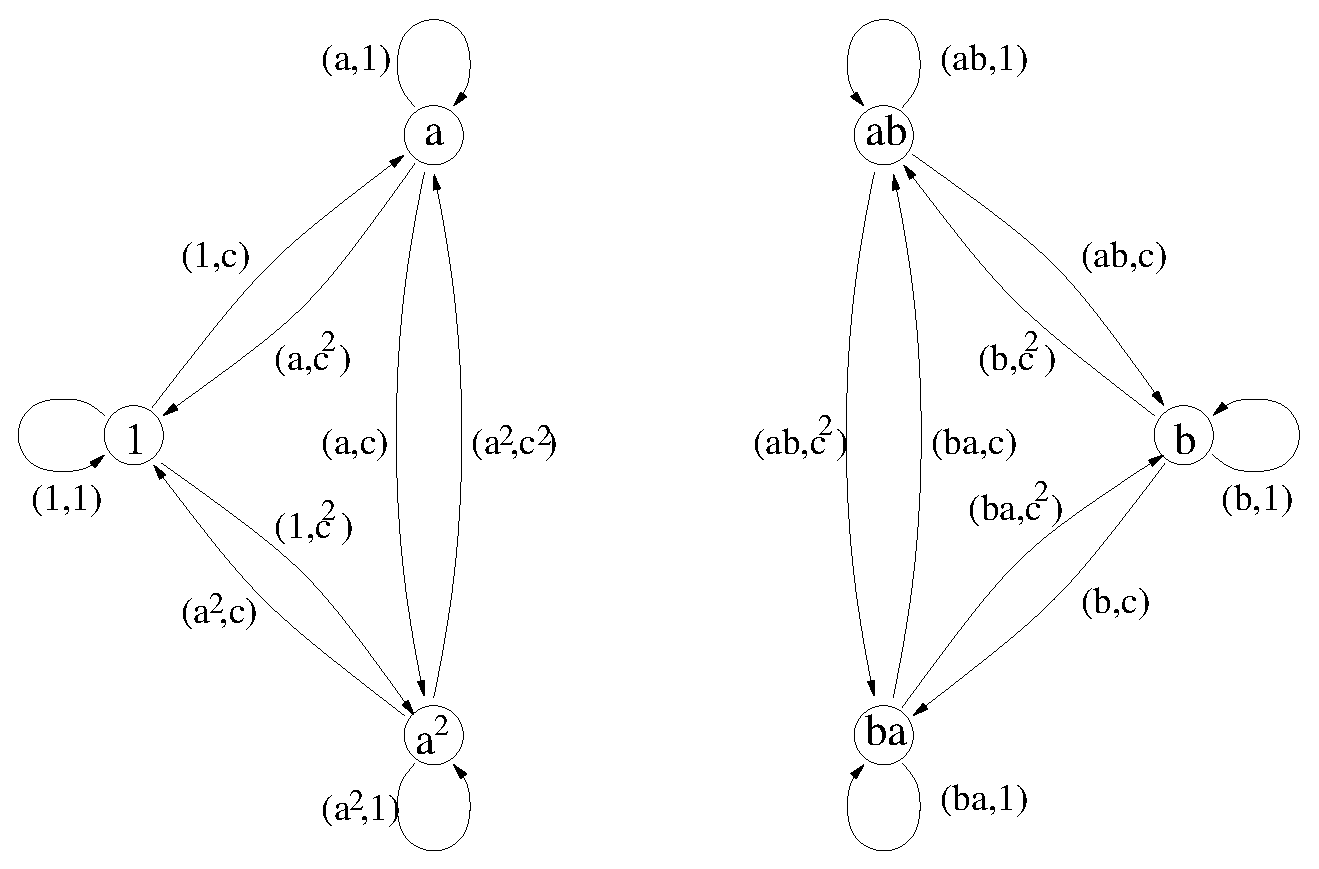
\includegraphics[scale = 0.60]{xmodcat1/s3ggpd.eps}
%% \input{s3ggpd.pstex_t} 
\end{center}

\noindent
\emph{We may compare the group multiplication with the groupoid multiplication
by calculating, for example,}
\begin{eqnarray*}
(a,c)(a^2,c) &=& (1,c^{a^2}c) ~=~ (1,c^2), \\
(a,c)*(a^2,c)     &=& (a,c)(a^2,1)^{-1}(a^2,c) ~=~ (a^4,c^{a^3}c) ~=~ (a,c^2).
\end{eqnarray*}
\end{example}

\begin{example} \label{ex:G18}
This example may be investigated in {\GAP} with the following corredpondence:
$$
a \mapsto (7,8,9),~ b \mapsto (8,9),~ c \mapsto (2,3)(4,5)
$$

{\small 
\begin{verbatim}
gap> G18 := GroupGroupoid( C18);
groupoid with 2 pieces:
1:  single piece groupoid with rays: < Group( [ ()>-()->() ] ), 
[ (), (7,8,9), (7,9,8) ], [ ()>-()->(), ()>-(4,6,5)->(7,9,8), 
  ()>-(4,5,6)->(7,8,9) ] >
2:  single piece groupoid with rays: < Group( [ (8,9)>-(2,3)(5,6)->(8,9) ] ), 
[ (8,9), (7,8), (7,9) ], [ (8,9)>-(2,3)(5,6)->(8,9), (8,9)>-(2,3)(4,5)->(7,8),
  (8,9)>-(2,3)(4,6)->(7,9) ] >
gap> piece2 := Pieces( G18 )[2];;
gap> obs2 := piece2!.objects;
[ (8,9), (7,8), (7,9) ]
gap> RaysOfGroupoid( piece2 );
[ (8,9)>-(2,3)(5,6)->(8,9), (8,9)>-(2,3)(4,5)->(7,8), 
  (8,9)>-(2,3)(4,6)->(7,9) ]
gap> elts2 := ElementsOfGroupoid( piece2 );;
gap> x := elts2[3];
[(8,9)>-(2,3)(4,6)->(7,9) : (8,9) -> (7,9)]
gap> y := elts2[8];
[(7,9)>-(1,3)(4,6)->(7,8) : (7,9) -> (7,8)]
gap> x*y;
[(8,9)>-(2,3)(4,5)->(7,8) : (8,9) -> (7,8)]
\end{verbatim}} 
\end{example} 


\newpage
%%%%%%%%%%%%%%%%%%%%%%%%%%%%%%%%%%%%%%%%%%%%%%%
\subsection{Regular Groupoids} \label{subs:reggpd} \index{regular groupoid} 

Let $\calX = (\partial : S \to R)$ be a precrossed module and let 
$\calC = (e;t,h : G \to R)$ be the associated precat$^1$-group 
where $G = R \ltimes S$ 
has multiplication $(r_1,s_1)(r_2,s_2) = (r_1r_2,s_1^{r_2}s_2)$ 
and inverse $(r,s)^{-1} = (r^{-1},(s^{-1})^{r^{-1}})$. 
The homomorphisms $e,t,h$ are given by 
$er = (r,1),~ t(r,s) = r,~ h(r,s) = r(\partial s)$. 

The associated group-groupoid $\calG$ has vertex set $R$ and arrows $G$ 
with the tail (source) and head (target) maps given by $t$ and $h$. 
Composition $*$ in $\calG$ is given by 
$$
(r_1,s_1) * (r_2,s_2) = (r_1,s_1)(r_2^{-1},1)(r_2,s_2) = (r_1,s_1s_2) 
$$ 
and is defined when $r_1(\partial s_1) = r_2$. 
The identity element in the object group at $r$ is $er = (r,1)$. 

\begin{defn} \label{defn:left-right-action}
Let $\calG$ be a groupoid with objects $R$ and arrows $G$. 
\begin{enumerate}[(i)]
\item
Maps $\rhd : R \times G \to G$ and $\lhd : G \times R \to G$ 
are respectively \emph{left} and \emph{right actions} of $R$ on $G$ 
if for all $q,r \in R$ and $g,h \in G$ 
\begin{itemize} 
\item 
$(qr) \rhd g = q \rhd (r \rhd g)$,~ $g \lhd (qr) = (g \lhd q) \lhd r$; 
\item
$q \rhd (g \lhd r) = (q \rhd g) \lhd r$; 
\item
$1 \rhd g = g = g \lhd 1$; 
\item
$t(r \rhd g) = r(tg)$,~ $t(g \lhd r) = (tg)r$,~ 
$h(r \rhd g) = r(hg)$,~ $h(g \lhd r) = (hg)r$; 
\item 
$r \rhd (g * g') = (r \rhd g) * (r \rhd g')$,~ 
$(g * g') \lhd r = (g \lhd r) * (g' \lhd r)$, 
whenever $g * g'$ is defined; 
\item 
$q \rhd er = e(qr) = eq \lhd r$. 
\end{itemize}
\item 
$\calG$ is \emph{semiregular} if $R$ is a monoid 
and if $\calG$ has left and right actions as in (i). 
\item
A semiregular $\calG$ is \emph{regular} if $R$ is a group. 
\end{enumerate}
\end{defn}

\begin{lem}
When $\calG$ is the group groupoid associated to a precat$^1$-group $\calC$, 
left and right actions are given by left and right multiplication:
$$
r \lhd g := (er)g, \qquad  g \rhd r := g(er).
$$
\end{lem}
\begin{pf}
We only verify the axioms for $\lhd$ since those for $\rhd$ follow similarly. 
\begin{eqnarray*}
g \lhd (qr) &=& g \lhd (eq)(er) = (g \lhd q)(er) = (g \lhd q) \lhd r; \\ 
q \rhd (g \lhd r) &=& q \rhd (g(er)) = (eq)g(er) 
                   =  ((eq)g) \lhd r = (q \rhd g) \lhd r; \\
g \lhd 1 &=& g(e1) = g; \\
t(g \lhd r) &=& t(g(er)) = (tg)(ter) = (tg)r; \\
h(g \lhd r) &=& h(g(er)) = (hg)(her) = (hg)r; \\
(g \lhd r)*(g' \lhd r) &=& (g(er))(eh(g(er)))^{-1}g'(er) 
     = g(er)(er)^{-1}(ehg)^{-1}g'(er) = (g*g') \lhd r; \\
eq \lhd r &=& (eq)(er) = e(qr). 
\end{eqnarray*}
\end{pf}

\begin{prop} 
Let $\calG$ be a semiregular groupoid. 
Then there are two everywhere defined binary operations on $G$ given by: 
\begin{eqnarray*}
g \circledcirc g' &=& (g \lhd tg') * (hg \rhd g'), \\ 
g \circledast g' &=& (tg \rhd g') * (g \lhd hg'). 
\end{eqnarray*} 
When $\calG$ is a regular groupoid both $\circledcirc$ and $\circledast$ 
make $G$ into a group with identity $e1$. 
\end{prop} 

Following on from the example above, when $\calG$ is a group groupoid, 
we find that $\circledcirc$ is just the multiplication in $G$. 
\begin{eqnarray*}
g \circledcirc g' &=& (g \lhd tg') * (hg \rhd g') \\
              &=& (g(etg'))*((ehg)g') \\ 
              &=& g(etg')(eh(g(etg')))^{-1}(ehg)g' \\ 
              &=& g(etg')((ehg)(etg'))^{-1}(ehg)g' \\ 
              &=& gg'. 
\end{eqnarray*} 
\noindent
The situation with $\circledast$ is a little more complicated: 
\begin{eqnarray*}
g \circledast g' &=& (tg \rhd g') * (g \lhd hg') \\ 
                 &=& ((etg)g')(eh((etg)g'))^{-1}(g(ehg') \\ 
                 &=& (etg)g')((etg)(ehg'))^{-1}g(ehg') \\ 
                 &=& (etg)g'(ehg')^{-1}(etg)^{-1}g(ehg'). 
\end{eqnarray*} 
Now $g'(ehg')^{-1} \in \ker h$ and $(etg)^{-1}g \in \ker t$. 
When $\calG$ is a cat$^1$-group these two products commute, 
so the expression reduces to $gg'$ and $\circledast$ is also 
just multiplication in $G$.



%%%%%%%%%%%%%%%%%%%%%%%%%%%%%%%%%%%%%%%%%%%
\subsection{$2$-groups} \label{subs:twogps}

Finally, we think of such a structure as a special case of a 
\index{$2$-category} \index{$2$-group} \index{$2$-cell} 
$2$-category, which has objects, morphisms, and $2$-\emph{cells}.
We follow the presentation in Subsection 1.2.3 of 
Forrester-Barker's thesis \cite{f-b-thesis}. 
For an introduction to $2$-groupoids, 
see Kamps and Porter \cite{kamps:port}.
(Note that a $2$-group is \emph{not} a special case of the group theorist's 
$p$-group, with $p=2$, but is a $2$-category with one object having all 
morphisms and $2$-cells invertible.)

The $2$-group $\calH$ associated to $\calX = (\partial : S \to R)$ has
\begin{itemize}
\item  a single object $\bullet$,
\item  morphisms $r \in R$,
\item  $2$-cells $(r,s) \in R \ltimes S$
       with tail $r$ and head $r(\partial s)$.
\end{itemize}
$$
\xy
\xymatrix{
   & & & \\
 \Downarrow (r,s)~= 
   & \bullet  \ar@/^5ex/[rr]^{r} 
              \ar@/_5ex/[rr]_{r(\partial s)} 
     & \Downarrow (r,s)
        & \bullet \\
   & & & \\
}
\endxy
$$

%\medskip
\noindent
Horizontal composition $(r_1,s_1) \sharpz (r_2,s_2)$ 
of $2$-cells is given by
$$
\xy
\xymatrix{
  & &  & & & & & & \\
  \bullet \ar@/^5ex/[rr]^{r_1} 
          \ar@/_5ex/[rr]_{r_1(\partial s_1)} 
  & \Downarrow (r_1,s_1)
    & \bullet \ar@/^5ex/[rr]^{r_2} 
              \ar@/_5ex/[rr]_{r_2(\partial s_2)} 
      & \Downarrow (r_2,s_2)
        & \bullet 
          & = 
            & \bullet \ar@/^5ex/[rr]^{r_1r_2} 
                      \ar@/_5ex/[rr]_{r_1(\partial s_1)r_2(\partial s_2)} 
              & \Downarrow (r_1r_2,{s_1}^{r_2}{s_2})
                & \bullet \\
  & & & & & & & & \\
}
\endxy
$$

%\medskip
\noindent
There is a unique \emph{horizontal identity} $2$-cell
$$
\xy
\xymatrix{
   & & & \\
 \Downarrow(1,1)~=
   & \bullet  \ar@/^5ex/[rr]^{1} 
             \ar@/_5ex/[rr]_{1} 
     & \Downarrow (1,1)
        & \bullet \\
   & & & \\
}
\endxy
$$

%\medskip
\noindent
Similarly, when $r_1(\partial s_1) = r_3$,
vertical composition $(r_1,s_1) \sharpo (r_3,s_3)$ 
of $2$-cells is given by
$$
\xy
\xymatrix{
  && && & & && \\
  && \Downarrow (r_1,s_1)
     && & & && \\
  \bullet \ar@/^15ex/[rrrr]^{r_1} 
          \ar[rrrr]^{r_1(\partial s_1)}
          \ar@/_15ex/[rrrr]_{r_1(\partial s_1)(\partial s_3)} 
  && && \bullet 
        &=& \bullet \ar@/^5ex/[rr]^{r_1} 
                    \ar@/_5ex/[rr]_{r_1(\partial(s_1s_3))} 
            & \Downarrow (r_1,s_1s_3)
             & \bullet \\
  && \Downarrow (r_1(\partial s_1),s_3)
     && & & && \\
  && && & & && \\
}
\endxy
$$

\medskip\noindent
For each $r \in R$ there is a \emph{vertical identity} $2$-cell 
$$
\xy
\xymatrix{
   & & & \\
 \Downarrow(r,1)~=
   & \bullet  \ar@/^5ex/[rr]^{r} 
             \ar@/_5ex/[rr]_{r} 
     & \Downarrow (r,1)
        & \bullet \\
   & & & \\
}
\endxy
$$
such that
$$
\Downarrow(r,1)\; \sharpo \Downarrow(r,s)\; 
                  \sharpo \Downarrow(r(\partial s),1)
~=~ \Downarrow(r,s).
$$

The \emph{horizontal inverse} and the 
\emph{vertical right inverse} of ~$\Downarrow(r,s)$~ 
are ~$\Downarrow(r^{-1},(s^{-1})^{r^{-1}})$~ and \\  
$\Downarrow(r(\partial s),s^{-1})$~ respectively.

Horizontal composition with vertical identities is called 
\emph{whiskering}. 
In diagrams it is often convenient to shrink ~$\Downarrow(q,1)$~ 
to a single arc, labelled $q$, as in the whiskering formlae:
$$
q_1 \sharpz \Downarrow(r,s) ~\sharpz~ q_2 
~=~ \Downarrow(q_1rq_2,{s}^{q_2}).
$$

\bigskip\noindent
The Peiffer condition for cat$^1$-groups establishes an 
\index{Peiffer condition} \index{interchange law} 
\emph{interchange law} for $\calH$,
$$
((r_1,s_1) \sharpz (r_2,s_2)) \sharpo ((r_3,s_3) \sharpz (r_4,s_4))
\quad = \quad
((r_1,s_1) \sharpo (r_3,s_3)) \sharpz ((r_2,s_2) \sharpo (r_4,s_4)) 
$$
for the well-defined composite 
when $r_1(\partial s_1) = r_3$ and $r_2(\partial s_2) = r_4$,
$$
\xy
\xymatrix{
  && && && && \\
  && \Downarrow (r_1,s_1)
     && && \Downarrow (r_2,s_2)
           && \\
  \bullet \ar@/^15ex/[rrrr]^{r_1} 
          \ar[rrrr]^{r_1(\partial s_1) = r_3}
          \ar@/_15ex/[rrrr]_{r_3(\partial s_3)} 
  && && \bullet \ar@/^15ex/[rrrr]^{r_2} 
                \ar[rrrr]^{r_2(\partial s_2) = r_4}
                \ar@/_15ex/[rrrr]_{r_4(\partial s_4)} 
        && && \bullet \\
  && \Downarrow (r_3,s_3)
     && && \Downarrow (r_4,s_4)
           && \\
  && && && && \\
}
\endxy
$$

\noindent
When this composite is defined, 
$$
    s_2{s_3}^{r_4}
~=~ s_2{s_3}^{r_2(\partial s_2)}
~=~ {s_3}^{r_2}s_2
$$
and the composite $2$-cell is
$$
\xy
\xymatrix{
   && && \\
   \bullet \ar@/^5ex/[rrrr]^{r_1r_2} 
           \ar@/_5ex/[rrrr]_{r_3(\partial s_3)r_4(\partial s_4)} 
   && \Downarrow (r_1r_2,(s_1s_3)^{r_2}s_2s_4)
      && \bullet \\
   && && \\
}
\endxy
$$
